\subsection{Probabilistic Skyline over Uncertain Data}
Given a d-dimensional data set, skyline query returns a set of points that are not dominated by any other points. A point \(p\) dominating a point \(q\) is denoted as \(p \prec p\); conversely, \(p \nprec p\) represents that \(p\) is not able to dominate \(q\). The domination relationship between points can be easily extended to group relationships easily. For example, \(p \prec D\) denotes that \(p\) dominates all points in \(D\). Similarly, \(D \prec p\) represents that all points in \(D\) dominates $p$. Next, let us introduce the components of uncertain datasets.

Let \(OS= \{O_{1},O_{2},\dots,O_{n}\}\) denotes the uncertain object set, and the number of objects is \(n\). We assume that an certain object has several instances, each of which is a d-dimensional attribute vector and has a probability to happen. Formally, \(O_{i}\) has an instance set \(O_{i} =\{p_{1},p_{2},\dots,p_{m}\}\), consisting of multiple \(d\)-dimensional instances with discrete probability density distribution of \(O_{i}\). Any instance \(p\)'s occurrence probability \(Pr(p)\) only depends on the object's \(pdf\)(probability density distribution), i.e., every object is independent of each other. For any object \(O\), we assume that \(\sum_{p\in O}Pr(p) = 1\). This is a realistic assumption adopted in many literatures~\cite{pei2007}~\cite{bohm2009}~\cite{kim2011} for analyzing uncertain data.

\begin{figure}
   \hspace{-35pt}
  \begin{minipage}[b]{0.80\linewidth}
    \centering
  	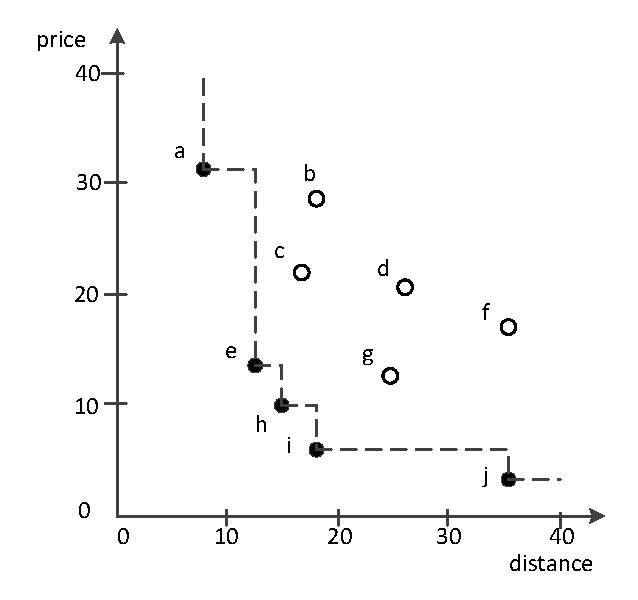
\includegraphics[width=0.8\linewidth]{figs/example.eps}
  	\par\vspace{-20pt}
  \end{minipage}%
  \hspace{-25pt}
  \begin{minipage}[b]{0.20\linewidth}
    \centering


  \begin{tabular}{|c|c|c|} \hline
  Obj & Instance & SkyProb \\ \hline \hline

  \multirow{3}{*}{P} & (6, 19) & 1 \\

  \cline{2-3}
    & (11, 17) & $\frac{4}{9}$ \\ 
  \cline{2-3}
    & (12, 8) & $\frac{2}{3}$  \\ \hline

  \multirow{3}{*}{Q} & (16, 7) & 1 \\

  \cline{2-3}
    & (21, 14) & $\frac{2}{9}$  \\ 
  \cline{2-3}
    & (11, 4) & 1  \\ \hline

  \multirow{3}{*}{W} & (8, 13) & 1 \\

  \cline{2-3}
    & (20, 9) & $\frac{2}{9}$  \\ 
  \cline{2-3}
    & (24, 3) & 1  \\ \hline
  \end{tabular}
  \hspace{-50pt}
\end{minipage}
\vspace{10pt}
\caption{Bla bla}
\label{fig:example}
\vspace{-10pt}
\end{figure}

Now we introduce the definition of Probabilistic Skyline, whose definition is quite different from traditional skyline. The goal of Probabilistic Skyline is to obtain the skyline probability \(SKYProb(O_{i})\) of one object \(O_{i}\), i.e., the likelihood that \(O_{i}\) becomes a skyline object. Given two objects \(O_{u}\) and \(O_{v}\), the probability that one instance \(p\) in \(O_{v}\) is dominated by another object \(O_{u}\) is:

\begin{equation}
\label{equ:1}
Pr(O_{u} \prec p) = \sum_{q \in O_{u}, \; q \prec p}Pr(q)
\end{equation}

Intuitively, the probability that \(p\) is a skyline instance for \(O_{u}\) is equal to that \(p\) is not dominate by \(O_{u}\), which can be represented by:

\begin{equation}
\label{equ:2}
Pr(O_{u} \nprec p) = 1 - \sum_{q \in P_{u}, \; q \prec p}Pr(q)
\end{equation}

Then we obtain the probability that \(p\) is not dominated for all objects in \(OS\) except $O_v$, which can be regarded as the likelihood of  $p$ to be a global skyline instance. As objects are independent of each other, \(SKYProb(p)\) (\( p \in O_{v}\)) is computed as follows:

\begin{equation}
\label{equ:3}
SKYProb(p) = \prod_{O_{u} \in OS, \; O_{u} \ne O_{v}}(1 - \sum_{q \in O_{u}, \; q \prec p}Pr(q))
\end{equation}

Finally, for object \(O_{v}\), we are able to obtain the skyline probability that \(O_{v}\) is a skyline object:
\begin{equation}
\label{equ_final}
SKYProb(O{v}) = \sum_{p \in O_{v}} Pr(p)SKY Prob(p)
\end{equation}

Given a threshold \(t\), we obtain an object set where $SKYProb(O_v)$ of every object is larger than $p$. That is,
\begin{equation}
\label{equ_threshold}
PSKY(OS) = \{ o \in OS|SKYProb(o)>t \}
\end{equation}

Take Figure~\ref{fig:example} as an example. We assume that all instances of an object are assigned the same weight. The instance skyline probability is firstly computed based on Equation~\ref{equ:3}. For $p_1$, no instance donimates it, then $SkyProb(p_1) = 1$; for $p_2$, $SkyProb(p_2) = 1* \frac{2}{3} * \frac{2}{3}$, since $w_1$ and $q_3$ dominates it. Then $SkyProb(P) = \frac{1}{3}( \frac{4}{9} + \frac{2}{3})$.

\subsection{MapReduce framework} %refer FEFEILI's EDBT12 paper
A typical MapReduce framework consists of two user-defined functions: map and reduce. For every record in the input data sets, map function will partition it into a sorted set of intermediate results. The reduce function fetches the data, from individual partition. Provided by the map function, Reduce process produces the final output data. The map and reduce function could be formally defined: \(map(k_{1},v_{1}) \rightarrow list(k_{2}, v_{2}) \) and \(reduce(k_{2},list(v_{2})) \rightarrow list(k_{3}, v_{3}) \).
